%%
%% Dit is een onderdeel van abi-instructie.tex
%%
\section{Fase 4 Scriptieafronding \& presentatie}

\subsection{Inleiding}
Ter afsluiting van het afstudeerproject bachelor
informatica, wanneer alle fasen afgerond en gedocumenteerd
zijn, stelt u het scriptieverslag samen bestaande uit
gezamenlijke en individuele bijdragen en houdt u een openbare
presentatie tijdens een offici\"ele academische zitting, gericht
op de opdrachtgever en de examinator.

De examinator zal vervolgens voor elke student een
afzonderlijke eindbeoordeling opstellen. Deze beoordeling zal
in het algemeen aansluiten bij de voorlopige deelbeoordelingen
die de begeleider gecommuniceerd heeft bij afronding van de
verschillende fasen.


\subsection{Doelstelling}
Deze fase vormt de afsluiting van het project. De beoordeling van deze fase
vindt plaats op basis van de presentatie en het scriptieverslag.
U stelt het scriptieverslag samen dat deels gezamenlijke teksten en deels
individuele teksten bevat, het verslag van individuele domeinanalyse.
U presenteert het project aan de opdrachtgever.

\subsection{Voorbereiding presentatie}
Er wordt pas definitief een eindpresentatie gepland wanneer duidelijk is dat
binnen afzienbare tijd alle documentatie (inclusief de individuele
scriptieverslagen) beschikbaar komt en ook van voldoende kwaliteit zal zijn.
Hiermee bestaat deze fase uit de volgende stappen, terugplannend vanaf de
beoogde presentatiedatum:

\par $\bullet$ (presentatiedatum - 4 weken): vaststellen of de documentatie
	    (van voldoende kwaliteit en volledig) binnen een maand beschikbaar kan zijn
\par $\bullet$ (presentatiedatum - 4 weken): vaststellen van een datum voor
	    de presentatie aan de opdrachtgever, de examinator, de begeleider en andere
	    belangstellenden
\par $\bullet$ (presentatiedatum - 4 weken): inplannen van een locatie voor
	    de afstudeeropdracht door het team en de begeleider, in afstemming met de
	    opdrachtgever en de examinator
\par $\bullet$ (presentatiedatum - 3 weken): informeren van de organisatie
	    (zowel via Studienet als ook via het OU Huisnet voor de staf van Informatica)
\par $\bullet$ (presentatiedatum - 2 weken): inleveren van de volledige
	    documentatie bij de begeleider
\par $\bullet$ (presentatiedatum - 1 week): feedback van de begeleider op de
	    volledige documentatie
\par $\bullet$ (presentatiedatum - 1 week): inleveren conceptpresentatie bij
	    de begeleider; u ontvangt hierop feedback voorafgaand aan de presentatie
\par $\bullet$ presentatiedatum: verzorgen presentatie
\par $\bullet$ presentatiedatum + 1 week: u ontvangt uw beoordeling op de
	    verschillende deelaspecten en het geheel en het tentamenbriefje.

U levert ten behoeve van stap 4 een beknopte tekst in waarin u het project
beschrijft ten behoeve van de uitnodiging. De presentatie duur ca 30 minuten
waarna een discussie volgt die maximaal een half uur kan duren.
De opzet van de presentatie is een gezamenlijk product. Elk teamlid dient bij de
presentatie aanwezig te zijn. Niet elk teamlid hoeft betrokken te zijn bij het
presenteren. maar dient wel deel te nemen aan de discussie.
De inhoud is voornamelijk gericht op de opdrachtgever en bevat vooral informatie
over het eindproduct, maar moet daarnaast ook een goede indruk geven over hoe
het project verlopen is.

\subsection{Onderdelen mijlpaalproduct}
\paragraph{Scriptieverslag}
U levert formeel een individueel scriptieverslag op als afronding van
het afstudeerproject bachelor informatica. Omdat u veel van het werk uitvoert
samen met uw teamgenoten zal het verslag merendeels uit gemeenschappelijke delen
bestaan. Alleen de hoofdstukken over de domeinen en technieken resulteert in een
individueel hoofdstuk. Het scriptieverslag, bestaat uit:

\begin{center}
\begin{tabular}{p{10em}p{25em}}
\hline
 titelblad &  	\par $\bullet$ titel van het verslag
		\par $\bullet$ Engelse titel
		\par $\bullet$ studentnaam, woonplaats en land
		\par $\bullet$ studentnummer
		\par $\bullet$ datum verslag
		\par $\bullet$ eventueel een figuur en/of bedrijfslogo
		\par $\bullet$ naam begeleider
		\par $\bullet$ naam examinator
		\par $\bullet$ "T61327 - Afstudeerproject bachelor informatica"
		\par $\bullet$ "Open Universiteit Nederland, faculteit Informatica"
 \\\hline
 korte samenvatting &  plusminus 250 woorden
 \\\hline
 introductie &  plusminus 3 A4 pagina's, gezamenlijk (mogelijke onderdelen:
context, vraagstelling etc)
 \\\hline
 requirements & plusminus 2 pagina's
 \\\hline
 algemeen overzicht domeinen en technieken & plusminus 2 pagina's
 \\\hline
    individueel verslag & onderzoek deeldomein en bijhorende technieken, plusminus
			5 pagina's
 \\\hline
    verslag analyse onderzoekcontext & plusminus 5 pagina's
 \\\hline
    beschrijving eindproduct & plusminus 15 pagina’s van wat is opgeleverd
 \\\hline
    procesverslag & voor zover relevant voor het begrijpen waarom het eindproduct
		in deze context de beste oplossing is: stappen met de beslissingen en de
		argumenten daarbij, plusminus 2 pagina's. Wellicht is dit geen getrouwe
		geschiedschrijving, maar een manier om de opdrachtgever en de examinator te
		laten begrijpen waarom dit een goed product is gegeven de kaders en
		doelstellingen
 \\\hline
    teamreflectie & op het project en de gekozen aanpak: wie heeft welke rollen
		    vervuld, hoe verliep het project, plusminus 2 pagina's
 \\\hline
    individueel verslag & persoonlijke ervaringen en leermomenten
 \\\hline
    conclusies en aanbevelingen & plusminus 2 pagina's, gezamenlijke tekst.
 \\\hline
\end{tabular}
\end{center}

Het scriptieverslag beslaat maximaal 50 pagina's exclusief bijlagen.
\paragraph{Eindpresentatie}
Een gezamenlijke presentatie, gericht op de opdrachtgever (ca. 30 minuten +
maximaal 30 min vragen, in de eerste plaats van de opdrachtgever).  Onderdelen
van de presentatie:
\begin{center}
\begin{tabular}{p{30em}}
    \par $\bullet$ zeer kort: wie zijn wij?
    \\\hline
    \par $\bullet$ hoe is de opdracht opgevat? Wat heeft de opdrachtgever nodig en wat beoogde
	    het team te leveren?
    \\\hline
    \par $\bullet$ de aanpak (kort proces, alleen voor zover van belang om het resultaat te
	kunnen beoordelen; zeker niet om een getrouw verslag van succes en falen en van
	individuele en groepsproblemen te beschrijven), vooral nadruk op de stappen met
	beslissingen en argumenten daarvoor
    \\\hline
    \par $\bullet$ wat was de bijdrage aan het onderzoeksproject?
    \\\hline
    \par $\bullet$ het resultaat besproken aan de hand van enkele
	relevante voorbeelden met plaatjes
    \\\hline
    \par $\bullet$ eventueel een vlekkeloos verlopende (of voorgekookte) demo
    \\\hline
    \par $\bullet$ verwijzing naar documentatie, code, etc.
    \\\hline
    \par $\bullet$ reflectie op het project en de gekozen aanpak:
	\par \qquad \leftpointright{} Wie heeft welke rollen vervuld?
	\par \qquad \leftpointright{} Hoe verliep het project?
    \\\hline
    \par $\bullet$ conclusies en aanbevelingen
	\par \qquad \leftpointright{} wat heb je bereikt?
	\par \qquad \leftpointright{} wat zou je nog kunnen doen?
    \\\hline
\end{tabular}
\end{center}

\subsection{Rol begeleider en examinator}
De begeleider en de examinator beoordelen uw mijlpaalproducten en geven een
eindbeoordeling waarbij elk onderdeel voldoende moet zijn.

\begin{center}
\begin{tabular}{ll}
\hline
{\bf fase} 		& {\bf beoordeling}\\\hline
fase 1 			& geen beoordeling\\
fase 2 			& groepsbeoordeling\\
fase 3a+ 		& individuele beoordeling\\
fasen 3b, 3c en 3d 	& groepsbeoordeling\\
fase 4   		& groepsbeoordeling\\
\hline
\end{tabular}
\end{center}


Bij de individuele beoordeling van fase 3a wordt in bijzondere gevallen de
bijdrage van het individuele teamlid aan de samenwerking van het gehele team
meegewogen, vandaar de aanduiding 3a+. Deze specifieke individuele beoordeling
wordt door de examinator in afstemming met de begeleider gegeven. Bij
de beoordeling wordt het onderstaande schema aangehouden. In het schema is
globaal en indicatief weergegeven hoe de beoordeling op de verschillende
aspecten plaatsvindt.

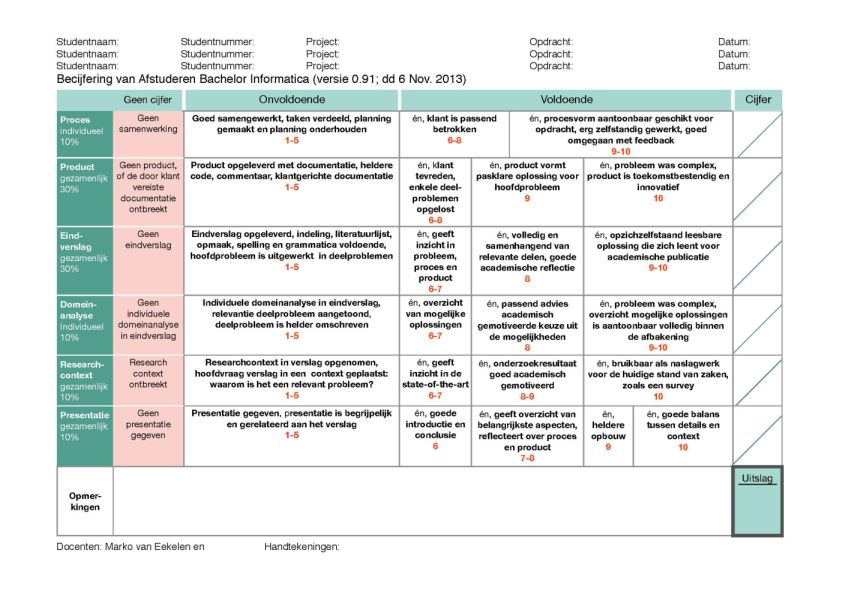
\includegraphics[width=17cm]{voorbeeld-ABI-cijfer}

\tablecaption{Beoordelingscriteria}
\tablehead{\hline {\bf eisen} & {\bf Criteria}\\}
\tabletail{\hline \multicolumn{2}{r}{Continues on next page}\\}
\tablelasttail{\hline}
\par{\tiny
\begin{center}
\begin{supertabular}{|l|p{30em}|}
\hline
\multicolumn{2}{|c|}{\emph{Presenteren}}\\\hline
Opbouw & De opbouw van de presentatie wordt duidelijk vermeld.
	Er wordt aangegeven welk teamlid welke rol in het project heeft vervuld en wie
	welk onderdeel van de presentatie zal verzorgen.
	Tijdens de presentatie is steeds duidelijk welke plaats het onderdeel in het
	geheel heeft.
\\\hline
Vormgeving & De bij de presentatie gebruikte hulpmiddelen (bv. Powerpoint) hebben een
	adequate vormgeving (kleurgebruik, hoeveelheid tekst per sheet, animaties, etc.)
\\hline
Communicatie & Er is duidelijkheid over de mogelijkheid tot het stellen van
	vragen, tijdens of na afloop van de presentatie. De vragen worden begrijpelijk beantwoord.
	De presentator(en) hebben de regie in handen.
\\\hline
Doelgroep & De presentatie is bedoeld voor de opdrachtgever, en moet dus aansluiten bij de
	achtergrondkennis van de opdrachtgever.
	De presentatie moet voor de opdrachtgever de relevante zaken over het  project
	duidelijk maken: wat is opgeleverd, hoe werkt het, welke onvolkomenheden bevat
	het systeem nog.
	De presentatie is ook goed te volgen voor stafleden van Informatica en
	gevorderde bachelor studenten.
\\\hline
\multicolumn{2}{|c|}{\emph{Klantgerichtheid}}\\\hline
Rol van de opdrachtgever & De contacten met de opdrachtgever over de presentatie verlopen qua inhoud en
	planning zodanig dat deze weet wat er van de presentatie verwacht mag worden.
\\\hline
Overdracht & De overdracht van het resultaat van het project aan de klant gebeurt op zo’n
	manier dat de klant de resultaten daadwerkelijk kan gaan gebruiken.
\\\hline
\multicolumn{2}{|c|}{\emph{Schrijven scriptie}}\\\hline
Taal & Het eindverslag is grammaticaal correct.
\\\hline
Precisie & De vereiste onderdelen komen voor in het verslag.
\\\hline
Structuur & De indeling van het verslag is helder.
	Er is samenhang tussen de tekstdelen.
\\\hline
Uitwerking probleemstelling & De probleemstelling is inhoudelijk
	verankerd in het onderzoek.
\\\hline
Presentatie vakinhoud & Het verslag maakt duidelijk hoe de opgeleverde producten van het project in
	relatie staan met de doelstelling van het project en de context van het onderzoek.
\\\hline
\end{supertabular}
\end{center}
}% tiny
